\documentclass[11pt,a4paper]{article}
\usepackage[margin=25mm]{geometry}
\usepackage{amsmath,amssymb}
\usepackage{booktabs}
\usepackage{hyperref}
\usepackage{xcolor}
\usepackage{listings}
\usepackage{tikz}
\usetikzlibrary{shapes,shapes.geometric,arrows.meta,positioning,fit,backgrounds}

\hypersetup{colorlinks=true,linkcolor=blue!60!black,citecolor=blue!60!black,urlcolor=blue!60!black}

\definecolor{codebg}{RGB}{245,245,245}
\definecolor{doneGreen}{RGB}{46,125,50}
\definecolor{wipYellow}{RGB}{245,160,0}
\definecolor{todoRed}{RGB}{180,40,40}

\lstdefinestyle{cpp}{
  backgroundcolor=\color{codebg},
  basicstyle=\ttfamily\small,
  keywordstyle=\color{blue!60!black}\bfseries,
  commentstyle=\color{gray},
  stringstyle=\color{red!60!black},
  numbers=left,numberstyle=\tiny\color{gray},numbersep=8pt,
  frame=single,rulecolor=\color{black!15},
  breaklines=true,tabsize=2,
  language=C++,
  morekeywords={override,final,noexcept,size_t}
}
\lstset{style=cpp}

\title{MiniANN Early Prototype: Mentor Meeting 1 Design Overview}
\author{Problem Statement 5: A Simple ANN Library in C++ \\ Team of 4 --- C++17, no external ML frameworks}
\date{\today}

\begin{document}
\maketitle

\begin{abstract}
This report documents the \textbf{initial-phase prototype} of MiniANN: a from-scratch,
object-oriented neural network library in modern C++17. At the Mentor Meeting~1 milestone
the architecture and 4-member module division are frozen for validation, and exactly one
functional module is complete: the \textbf{polymorphic activation subsystem}
(\texttt{IActivation} with \texttt{Sigmoid}, \texttt{Tanh}, \texttt{ReLU}).
A minimal forward-only skeleton (\texttt{Neuron} $\to$ \texttt{Layer} $\to$
\texttt{NeuralNetwork} $\to$ \texttt{predict}) proves the composition design compiles and runs,
while training, dataset ingestion, and evaluation exist only as explicit
\texttt{logic\_error} stubs marking each member's future work. We explain the purpose of this
snapshot, why each design choice was made, what the code does module by module, how it was
verified, and what is deliberately left for the full MVP (cf.\ \texttt{MiniANN\_MVP/}).
\end{abstract}

\tableofcontents
\newpage

% ============================================================
\section{Purpose of this prototype}
% ============================================================
The Meeting~1 goal, as stated in the brief, is to \textbf{validate architecture, confirm module
division, and gather suggestions} --- not to show a learning network. Concretely this report must
convince a mentor of three things:
\begin{enumerate}
  \item The team understands what an ANN is mathematically ($z = w\cdot x + b$,
    $\mathit{output}=\mathit{activation}(z)$) and can map each concept to a class or interface.
  \item The proposed composition hierarchy and separation of training from the model are sound
    Object-Oriented Design.
  \item Work can proceed in parallel without interface drift, because headers are frozen and
    unfinished parts fail loudly instead of silently.
\end{enumerate}
Hence this prototype is \textbf{intentionally incomplete}: it compiles, its activation tests pass,
its forward demo runs, and its training stub throws. An XOR network at this stage outputs
essentially random values ($\approx 0.43$ for every input) --- that \emph{is} the expected result,
because backpropagation does not exist yet.

\subsection{Why clarity over speed}
Production frameworks (PyTorch, TensorFlow) and matrix libraries (Eigen, BLAS) are banned by the
brief. Every multiplication is a visible loop over \texttt{std::vector<double>}. The payoff is
pedagogical: a reader can trace a prediction from \texttt{NeuralNetwork::predict} through
\texttt{Layer::forward} to \texttt{Neuron::forward} to \texttt{IActivation::activate} with no
hidden machinery. Performance, GPU support, and autograd are explicitly out of scope.

\subsection{Relation to the full MVP}
\texttt{MiniANN\_Early/} is the starting point; \texttt{MiniANN\_MVP/} is the destination. The
MVP adds: \texttt{backward()}/gradient accumulation, Xavier/He initialization, SGD and Adam,
\texttt{Trainer::fit} with mini-batches, RFC-4180 CSV loading, accuracy/confusion-matrix metrics,
17-digit model serialization, console logging, and 100\% XOR/Iris demos. Nothing in the early
headers contradicts the MVP --- the MVP only \emph{fills in} the stubs defined here.

% ============================================================
\section{What the prototype does (and does not do)}
% ============================================================
Table~\ref{tab:scope} is the contract. ``DONE'' means compiled, tested, and demoed.
``STUB'' means the header exists so members can compile against it, but every call throws
\texttt{std::logic\_error("Meeting 1: \dots\ not implemented")}.

\begin{table}[h]
\centering
\caption{Meeting~1 scope: done vs.\ planned.}\label{tab:scope}
\begin{tabular}{@{}lll@{}}
\toprule
Module (owner) & Status & Evidence \\
\midrule
Common types (\texttt{types.hpp}) & DONE & \texttt{Vector}, \texttt{Matrix} aliases \\
Activations (\texttt{activation.hpp}) & DONE & \texttt{test\_activation.exe} passes \\
Neuron forward (M2) & DONE (forward only) & \texttt{forward\_demo.exe} runs \\
Layer / Network forward (M1) & DONE (forward only) & dim check throws \texttt{invalid\_argument} \\
\texttt{MSELoss::compute} (M3) & PARTIAL & value only, no gradient yet \\
\texttt{SGD::step}, backprop, \texttt{Trainer} (M3) & STUB & throws, demo catches it \\
\texttt{Dataset::loadCSV}, \texttt{accuracy} (M4) & STUB & throws \\
Serialization, logging, CLI demos (M4) & NOT STARTED & absent by design \\
\bottomrule
\end{tabular}
\end{table}

In particular the program \textbf{cannot learn}: there is no loss gradient, no weight update, no
data loader, and no metric. The forward demo computes an MSE \emph{value} purely to show the loss
interface shape, then deliberately calls the optimizer stub to prove it throws.

% ============================================================
\section{How we did it: module by module}
% ============================================================

\subsection{Common types}
\texttt{namespace miniann} holds \texttt{using Vector = std::vector<double>} and
\texttt{using Matrix = std::vector<std::vector<double>>}. Every later header includes only
\texttt{types.hpp} plus what it needs, so physical dependencies mirror the logical diagram in
Fig.~\ref{fig:composition}. No raw \texttt{new}/\texttt{delete} anywhere; memory is owned by
\texttt{vector} and \texttt{unique\_ptr}.

\subsection{Activation subsystem (the completed piece)}
The brief's interface is reproduced verbatim:
\begin{lstlisting}
class IActivation {
public:
    virtual ~IActivation() = default;
    virtual double activate(double z) const = 0;
    virtual double derivative(double z) const = 0;
};
class Sigmoid : public IActivation {};
class Tanh : public IActivation {};
class ReLU : public IActivation {};
\end{lstlisting}
Why an abstract base? Each neuron must hold \emph{some} non-linearity without knowing which one
at compile time. A \texttt{unique\_ptr<IActivation>} member plus virtual dispatch gives exactly
that: the same \texttt{Neuron::forward} line \texttt{activation\_->activate(z)} executes
sigmoid, tanh, or ReLU depending on what the factory closure injected. The derivative is declared
now --- even though no caller uses it yet --- because backpropagation will need $f'(z)$ evaluated
at the \emph{pre-activation} $z$, and freezing that signature in Meeting~1 prevents the classic
$z$-vs-$a$ integration bug later.

Mathematics implemented in \texttt{src/activation.cpp}:
\begin{equation}
\sigma(z)=\frac{1}{1+e^{-z}},\quad \sigma'(z)=\sigma(z)(1-\sigma(z)),\qquad
\tanh'(z)=1-\tanh^2(z),\qquad
\mathrm{ReLU}(z)=\max(0,z),\; \mathrm{ReLU}'(z)=\mathbf{1}_{z>0}.
\end{equation}
Uniform initialization ($w\sim U(-1,1)$, $b\sim U(-0.5,0.5)$) is used for now; Xavier/He variance
preservation is explicitly deferred to the training phase.

\subsection{Neuron: the smallest unit}
\begin{lstlisting}
class Neuron {
public:
    Neuron(std::size_t numInputs, std::unique_ptr<IActivation> act,
           std::mt19937& rng);
    double forward(const Vector& inputs); // z = w.x + b, return activation(z)
    const Vector& weights() const { return weights_; }
    double bias() const { return bias_; }
private:
    Vector weights_; double bias_ = 0.0;
    std::unique_ptr<IActivation> activation_;
};
\end{lstlisting}
Encapsulation is strict: weights and bias are private, readable but not writable from outside
(no public data, no setters yet --- setters arrive with the serializer in the MVP). There is no
cached $z$, no $\delta$, no gradient buffer, because nothing computes gradients yet. The
constructor takes the RNG by reference so the network seed controls the whole experiment.

\subsection{Layer and network: composition over inheritance}
A \texttt{Layer} owns \texttt{std::vector<Neuron>} and maps \texttt{forward} over it; a
\texttt{NeuralNetwork} owns \texttt{std::vector<Layer>} and chains them:
\begin{lstlisting}
Vector Layer::forward(const Vector& inputs) {
    Vector out; out.reserve(neurons_.size());
    for (auto& n : neurons_) out.push_back(n.forward(inputs));
    return out;
}
Vector NeuralNetwork::predict(const Vector& input) {
    Vector out = input;
    for (auto& l : layers_) out = l.forward(out);
    return out;
}
\end{lstlisting}
\texttt{addLayer(numNeurons, numInputs, makeAct)} validates
\texttt{numInputs == previous\_layer\_size} and throws \texttt{invalid\_argument} otherwise ---
this is Member~1's core contribution at this stage. A small factory helper
(\texttt{useSigmoid()}/\texttt{useTanh()}/\texttt{useReLU()} returning
\texttt{std::function<std::unique\_ptr<IActivation>()>}) lets each layer pick its own
non-linearity without the network knowing concrete types. Crucially, \texttt{predict} is the
\emph{only} computation entry point; there is no \texttt{backward()}, no \texttt{zeroGradients()},
no training hook inside the model. That absence is the design statement: the network answers
``what am I?'', the future trainer will answer ``how do I learn?''.

\subsection{Training and data stubs (honest placeholders)}
\texttt{include/miniann/training.hpp} freezes the intended Member~3 interface
(\texttt{ILoss}, \texttt{MSELoss::compute}, \texttt{IOptimizer}, \texttt{SGD}) while
\texttt{src/training.cpp} implements only the pure value computation and makes \texttt{SGD::step}
throw. Likewise \texttt{dataset.hpp} offers \texttt{add()}/accessors but \texttt{loadCSV} and the
free \texttt{accuracy()} throw. This pattern --- \textbf{compilable headers, throwing bodies} ---
lets all four members build against the same headers in parallel while making unfinished work
impossible to mistake for working code (the forward demo catches the throw on purpose).

% ============================================================
\section{Architecture diagrams}
% ============================================================

\begin{figure}[h]
\centering
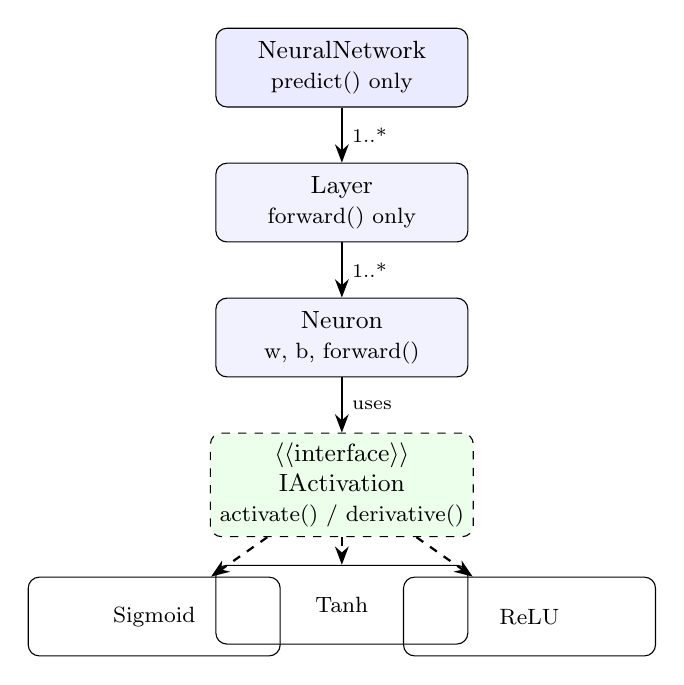
\begin{tikzpicture}[
  box/.style={draw,rounded corners,minimum width=3.2cm,minimum height=1.0cm,align=center,font=\small},
  iface/.style={draw,dashed,rounded corners,minimum width=3.2cm,minimum height=1.0cm,align=center,font=\small},
  arrow/.style={-{Stealth},thick}
]
\node[box,fill=blue!8] (net) {NeuralNetwork\\{\footnotesize predict() only}};
\node[box,fill=blue!5,below=0.7cm of net] (layer) {Layer\\{\footnotesize forward() only}};
\node[box,fill=blue!5,below=0.7cm of layer] (neuron) {Neuron\\{\footnotesize w, b, forward()}};
\node[iface,fill=green!8,below=0.7cm of neuron] (iact) {$\langle\langle$interface$\rangle\rangle$\\IActivation\\{\footnotesize activate() / derivative()}};
\node[box,below left=0.5cm and -0.9cm of iact,font=\footnotesize] (sig) {Sigmoid};
\node[box,below=0.35cm of iact,font=\footnotesize] (tanh) {Tanh};
\node[box,below right=0.5cm and -0.9cm of iact,font=\footnotesize] (relu) {ReLU};
\draw[arrow] (net) -- node[right,font=\scriptsize]{1..*} (layer);
\draw[arrow] (layer) -- node[right,font=\scriptsize]{1..*} (neuron);
\draw[arrow] (neuron) -- node[right,font=\scriptsize]{uses} (iact);
\draw[arrow,dashed] (iact) -- (sig);
\draw[arrow,dashed] (iact) -- (tanh);
\draw[arrow,dashed] (iact) -- (relu);
\end{tikzpicture}
\caption{Composition hierarchy (done). The model owns forward prediction only; no training edge exists yet.}\label{fig:composition}
\end{figure}

\begin{figure}[h]
\centering
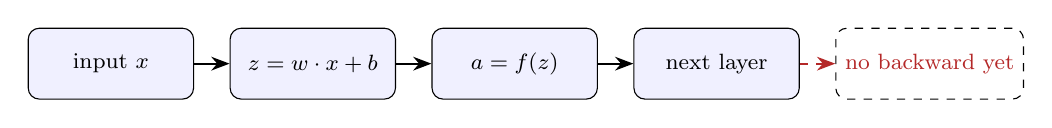
\begin{tikzpicture}[
  stage/.style={draw,rounded corners,minimum width=2.1cm,minimum height=0.9cm,align=center,font=\footnotesize,fill=blue!6},
  arrow/.style={-{Stealth},thick}
]
\node[stage] (x) {input $x$};
\node[stage,right=0.45cm of x] (z) {$z=w\cdot x+b$};
\node[stage,right=0.45cm of z] (qa) {$a=f(z)$};
\node[stage,right=0.45cm of qa] (nxt) {next layer};
\node[draw,dashed,rounded corners,right=0.45cm of nxt,minimum width=2.1cm,minimum height=0.9cm,align=center,font=\footnotesize,text=todoRed] (nope) {no backward yet};
\draw[arrow] (x) -- (z);
\draw[arrow] (z) -- (qa);
\draw[arrow] (qa) -- (nxt);
\draw[arrow,dashed,color=todoRed] (nxt) -- (nope);
\end{tikzpicture}
\caption{Forward data flow (solid = implemented; dashed red = explicitly absent in Meeting~1).}\label{fig:forward}
\end{figure}

\begin{figure}[h]
\centering
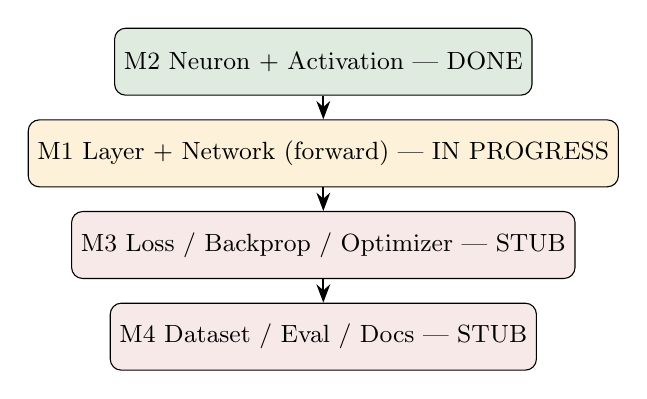
\begin{tikzpicture}[
  mod/.style={draw,rounded corners,minimum width=4.2cm,minimum height=0.85cm,align=left,font=\small},
  arrow/.style={-{Stealth},thick}
]
\node[mod,fill=doneGreen!15] (m2) {M2 Neuron + Activation --- DONE};
\node[mod,fill=wipYellow!15,below=0.3cm of m2] (m1) {M1 Layer + Network (forward) --- IN PROGRESS};
\node[mod,fill=todoRed!10,below=0.3cm of m1] (m3) {M3 Loss / Backprop / Optimizer --- STUB};
\node[mod,fill=todoRed!10,below=0.3cm of m3] (m4) {M4 Dataset / Eval / Docs --- STUB};
\draw[arrow] (m2) -- (m1);
\draw[arrow] (m1) -- (m3);
\draw[arrow] (m3) -- (m4);
\end{tikzpicture}
\caption{Module ownership and completion state. Color encodes status, arrows encode planned integration order.}\label{fig:modules}
\end{figure}

The roadmap (Fig.~\ref{fig:modules} read bottom-up as time) is: 1.~Design (this report),
2.~Core Components (finish forward + dimensions), 3.~Training (gradients, optimizer),
4.~Integration and Testing (datasets, metrics, demos). Each phase adds code without changing
frozen signatures.

% ============================================================
\section{Verification: proving ``done'' and proving ``not done''}
% ============================================================
Build (no CMake required):
\begin{lstlisting}[language=bash]
cd MiniANN_Early
.\build.bat
.\test_activation.exe
.\activation_demo.exe
.\forward_demo.exe
\end{lstlisting}
Expected output (abbreviated):
\begin{lstlisting}
Build OK (Meeting 1: activation + forward only)
MEETING1 ACTIVATION TESTS PASS
MiniANN Meeting 1: activation module
  z=0.0 -> 0.5000 (deriv 0.2500)
sigmoid(0)=0.5000 (expect 0.5)
relu(-2)=0.0000 (expect 0)
MiniANN Meeting 1: forward-only XOR (UNTRAINED)
  [0,0] -> 0.4371 (mse-vs-0 0.1910)
  [1,1] -> 0.4317 (mse-vs-0 0.1864)
training stub correctly throws: Meeting 1: SGD::step not implemented ...
\end{lstlisting}
\texttt{test\_activation} asserts $\sigma(0)=0.5$, $\sigma'(0)=0.25$, $\tanh(0)=0$,
$\mathrm{ReLU}(-2)=0$, plus a virtual-dispatch check through \texttt{const IActivation*}. The
forward demo builds a 2-2-1 tanh/sigmoid net (seed 42) and evaluates the four XOR corners
\emph{without training}: outputs cluster near $0.43$ regardless of input, confirming the plumbing
works and learning is absent. The caught \texttt{logic\_error} is a positive test --- it proves a
reviewer cannot accidentally believe training exists.

% ============================================================
\section{Limitations and path to the full MVP}
% ============================================================
Everything below is out of scope for this snapshot and appears only as a stub or not at all:
backpropagation and gradient accumulation, Xavier/He initialization, SGD/Adam stepping,
mini-batch \texttt{Trainer::fit}, CSV ingestion and splits, accuracy/confusion-matrix metrics,
\texttt{setprecision(17)} serialization with \texttt{MINIANN 1} magic, logging, and any demo that
learns (XOR at 100\%, Iris). The upgrade path is additive: implement \texttt{Neuron::backward}
($\delta = \partial L/\partial a\cdot f'(z)$, accumulate $\nabla w$), \texttt{Layer::backward}
($\partial L/\partial a_{\mathrm{prev}} = W^T\delta$ with pre-step weights),
\texttt{NeuralNetwork::backward}, the optimizer, and the data layer --- without touching the
activation headers frozen here.

% ============================================================
\section{Appendix: mentor questions and build notes}
% ============================================================
We ask: (1)~is the training-outside-network split correct; (2)~is the 4-member division
balanced; (3)~are activations, losses, optimizers, and metrics the right OOP seams? Build flags
are \texttt{-std=c++17 -Wall -Wextra -Wpedantic}, zero raw \texttt{new}/\texttt{delete},
\texttt{const}-correct accessors, \texttt{PascalCase} classes / \texttt{I}-interfaces /
\texttt{camelCase} methods / trailing-\texttt{\_} members. Reproduce with
\texttt{cmake -B build -S . \&\& cmake --build build} or \texttt{build.bat}.

\end{document}
